\documentclass{article}
\usepackage{pythonhighlight}
\usepackage{graphicx}
\usepackage{ctex}
\usepackage[left=3cm,top=3cm,right=3cm]{geometry}
\usepackage{hyperref}
% TITLE PAGE CONTENT %%%%%%%%%%%%%%%%%%%%%%%%
%%%%%%%%%%%%%%%%%%%%%%%%%%%%%%%%%%%%%%%%%%%%%
\newcommand{\labno}{09}
\newcommand{\labtitle}{EE208 Hadoop Streaming}
\newcommand{\authorname}{周李韬}
\newcommand{\studentno}{518030910407}
\newcommand{\classno}{F1803016}
% END TITLE PAGE CONTENT %%%%%%%%%%%%%%%%%%%%


\begin{document}

\begin{center}
{\LARGE \textsc{Laboratory No. \labno:} \\ \vspace{4pt}}
{\Large \textsc{\labtitle} \\ \vspace{4pt}} 
\rule[13pt]{\textwidth}{1pt} \\ \vspace{15pt}
{\large By: \authorname \\ \vspace{10pt}
No. \studentno \\ \vspace{10pt}
SJTU \classno \\ \vspace{10pt}
\today \vspace{20pt}}
\end{center}



\section{实验准备}

\subsection{实验环境}
\begin{itemize}
\item\textbf{Environment} Ubuntu 16.04 (on Virtual Machine)
\item\textbf{Tools} Hadoop 2.7.3, openjdk-8-jdk
\end{itemize}

\subsection{实验目的}

本实验中,我们需要借助Hadoop中的Map-Reduce模型,实现分布式地计算文章中单词平均长度,计算一张图中的PageRank。

\subsection{实验原理}

Map-Reduce的原理在上一次实验中已阐述。简单来说,Map对输入数据进行运算后,会产生一系列中间变量,随后Reduce函数对中间变量进行运算,得到输出结果。其中,Map和Reduce过程需要能够实现分布式运算。在Hadoop的MapReduce模型中,在Map和Reduce之间,会有一次对数据的排序过程,利用这一功能,Map结果将会按照数据的Key排序,从而使下一步Reduce提供帮助。

\paragraph{计算单词平均长度}

我们可以采用和WordCount Example类似的思想解决计算单词平均长度的问题。对读入的每个单词,我们将其通过Map函数产生(首字母,单词长度,单词个数(初始值为1))的记录,在Reduce函数中,对相同首字母的记录做合并操作,将单词长度、单词个数进行累加,最后输出单词长度和单词个数之商,就得到了所有首字母开头的单词的平均长度分布。


\paragraph{计算PageRank}
本实验中,我们通过迭代的方式计算图的PageRank。在一次迭代中,我们通过以下公式计算一个点的PageRank。
$$ PageRank(v) = \sum_{(u,v)\in \mathbf{G}} {\frac{PageRank(u)}{OutDegree(u)}}$$

数学中可以证明,在对所有节点进行该运算后,一次迭代运算的结果中所有节点的PageRank之和仍为1,且在连通性较好的情况下中,多次迭代能够收敛到页面真实的PageRank值。

在分布式实现方面,我们假设图是以邻接表的形式存储在文本文件中的,由于图的结构在运算过程中只会被读取,不会被修改,因此我们考虑在实验中将图作为一组静态数据,在输入时图结构会被Map函数读入参与运算,在Reduce过程中,参与运算后就会被消去。在下一次迭代时,再重新通过Map函数读取静态的图结构邻接表参与PageRank的运算。

与静态的邻接表相对的是存储每个节点PageRank的PageRank向量。我们通过一个(节点,PageRank)的列表存储该数据。在Map过程中,我们对每一个点,可以通过图邻接表读取它的所有出点,通过PageRank向量读取节点的PageRank值,我们将PageRank除以该节点邻接表的长度,使得该节点的PageRank平均分配给它的每一个出点。我们将出点和由当前节点贡献的rank值作为中间值返回。

由于在执行Reduce之前,Hadoop会对各中间值按照KEY进行排序,因此相同KEY的(节点,subRank)记录会被相邻排列。不难通过Reduce过程将相同节点的Rank值相加合并。最终的输出就是经过一次迭代后的PageRank向量。

在迭代的实现方面,我们使用bash,循环调用Hadoop中的Map-Reduce命令,每一次迭代的输出就是下一次迭代的输入,直到达到一定的迭代次数退出,输出各节点最终的PageRank值。

\section{实验步骤}

\subsection{计算单词平均长度}


\subsection{计算$\pi$}

\begin{figure}[htbp]
\centering
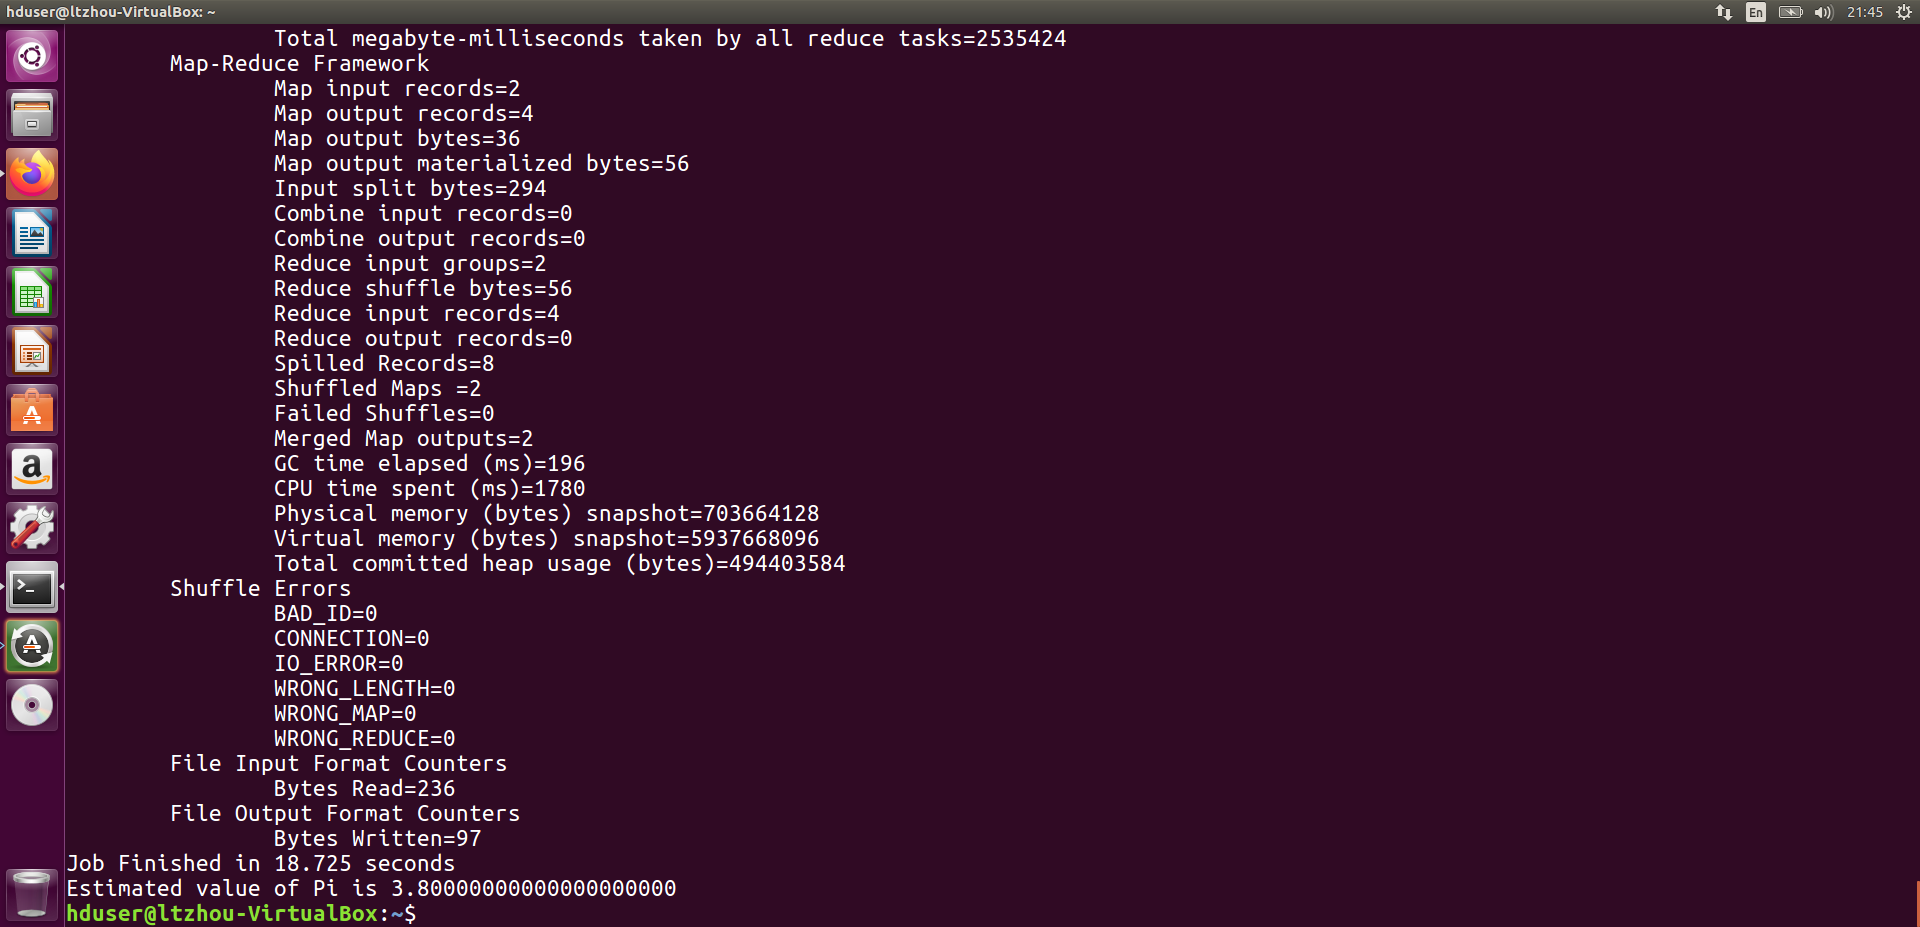
\includegraphics[width=13.5cm]{img/2-10.png}
\caption{Map=2, Sample=10时运行结果实例}
\label{fig:2-10}
\end{figure}

\begin{figure}[htbp]
\centering
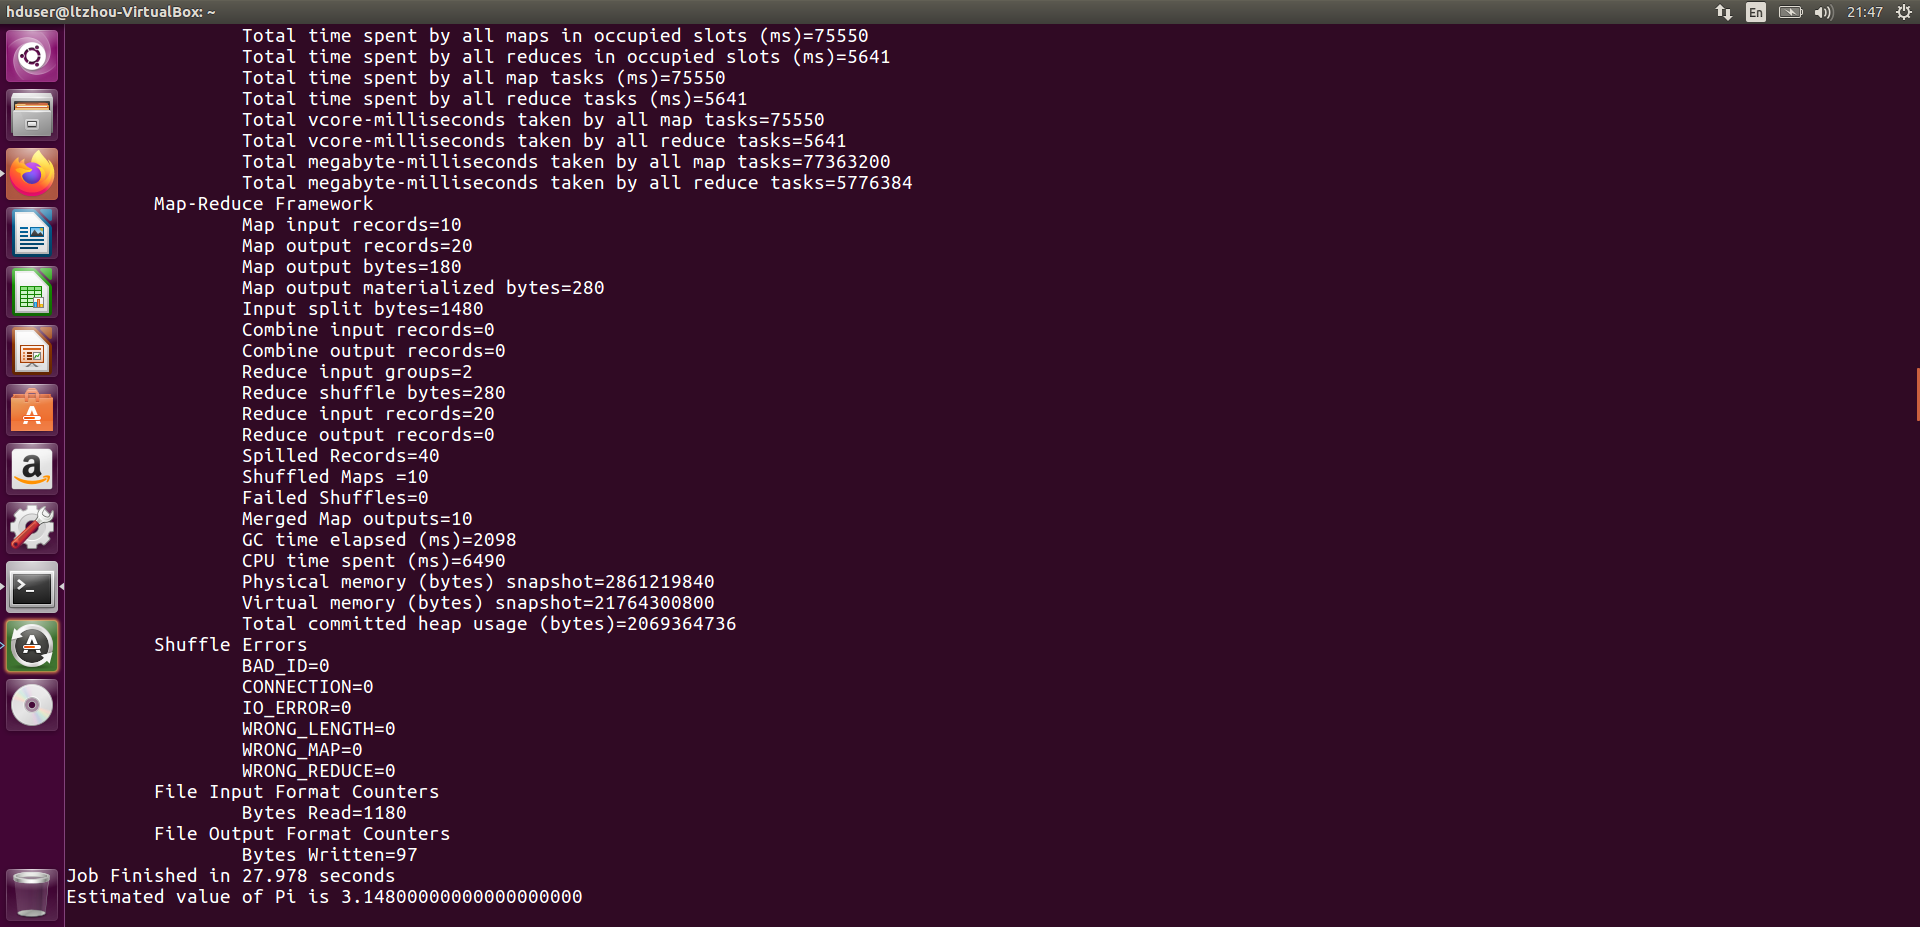
\includegraphics[width=13.5cm]{img/10-100.png}
\caption{Map=10, Sample=100时运行结果实例}
\label{fig:2-10}
\end{figure}



\section{实验总结}
\paragraph{概述}
本实验中,我们完成了Hadoop的安装、配置,并通过实验分布式地计算了$\pi$的估计值。

\paragraph{感想}
通过本次实验的学习,我体会到到了分布式运算带来的运算效率提升。分布式运算能够帮助我们更充分地利用、扩展现有的硬件资源,带来性能的提升。我也通过实验的尝试,学习了MAP-REDUCE模型的思想,希望这次实验的学习能够为以后的LAB做好铺垫。


\end{document}

